%% AMS-LaTeX Created with the Wolfram Language : www.wolfram.com



\begin{doublespace}
\noindent\(\pmb{\text{clear}[f,g]}\)
\end{doublespace}

\begin{doublespace}
\noindent\(\text{clear}[f,g]\)
\end{doublespace}

This is the Objective function that we now declare (f) note that we use $x_2=y$:

\begin{doublespace}
\noindent\(\pmb{f[\text{x$\_$},\text{y$\_$}]\text{:=}2*x^2+2*x*y+y^2-10*x-10*y}\)
\end{doublespace}

Now we declare the constraints by separate.

\begin{doublespace}
\noindent\(\pmb{\text{g1}[\text{x$\_$},\text{y$\_$}]\text{:=} x^2+y^2-5}\)
\end{doublespace}

\begin{doublespace}
\noindent\(\pmb{\text{g2}[\text{x$\_$},\text{y$\_$}]\text{:=} 2x+y-6}\)
\end{doublespace}

Now we solve all the possible Lagrangians.\\
First Assume no constraint is Binding

\begin{doublespace}
\noindent\(\pmb{\text{Solve}[\text{Grad}[f[x,y],\{x,y\}]\text{==} \{0,0\},\{x,y\}]}\)
\end{doublespace}

\begin{doublespace}
\noindent\(\pmb{\{\{x\to 0,y\to 5\}\}}\)
\end{doublespace}

Which is a solution for the unconstrained problem. Let{'}s see if it satisfies the constraints:

\begin{doublespace}
\noindent\(\pmb{\text{g1}[0,5]}\)
\end{doublespace}

\begin{doublespace}
\noindent\(20\)
\end{doublespace}

And it was supposed to be lower or equal than zero! So it violates the first constraint, and (0,5) cannot be a solution.\\
Let{'}s go on with using the first constraint, and given that the solution might have some Complex numbers we will constraint it to the Real Numbers:

\begin{doublespace}
\noindent\(\pmb{\text{Solve}[\{\text{Grad}[f[x,y],\{x,y\}]==\lambda *\text{Grad}[\text{g1}[x,y],\{x,y\}],\text{g1}[x,y]==0\},\{x,y,\lambda \},\text{Reals}]}\)
\end{doublespace}

\begin{doublespace}
\noindent\(\left\{\{x\to 1,y\to 2,\lambda \to -1\},\left\{x\to \left(5+\frac{5^{2/3}}{\left(3 \left(-9+4 \sqrt{6}\right)\right)^{1/3}}-\frac{\left(5
\left(-9+4 \sqrt{6}\right)\right)^{1/3}}{3^{2/3}}\right)/\left(\frac{16}{7}+\frac{93}{70} \left(-\frac{5^{2/3}}{\left(3 \left(-9+4 \sqrt{6}\right)\right)^{1/3}}+\frac{\left(5
\left(-9+4 \sqrt{6}\right)\right)^{1/3}}{3^{2/3}}\right)-\frac{29}{28} \left(-\frac{5^{2/3}}{\left(3 \left(-9+4 \sqrt{6}\right)\right)^{1/3}}+\frac{\left(5
\left(-9+4 \sqrt{6}\right)\right)^{1/3}}{3^{2/3}}\right)^2+\frac{137}{280} \left(-\frac{5^{2/3}}{\left(3 \left(-9+4 \sqrt{6}\right)\right)^{1/3}}+\frac{\left(5
\left(-9+4 \sqrt{6}\right)\right)^{1/3}}{3^{2/3}}\right)^3-\frac{23}{175} \left(-\frac{5^{2/3}}{\left(3 \left(-9+4 \sqrt{6}\right)\right)^{1/3}}+\frac{\left(5
\left(-9+4 \sqrt{6}\right)\right)^{1/3}}{3^{2/3}}\right)^4+\frac{17 \left(-\frac{5^{2/3}}{\left(3 \left(-9+4 \sqrt{6}\right)\right)^{1/3}}+\frac{\left(5
\left(-9+4 \sqrt{6}\right)\right)^{1/3}}{3^{2/3}}\right)^5}{1400}\right),y\to -\frac{5^{2/3}}{\left(3 \left(-9+4 \sqrt{6}\right)\right)^{1/3}}+\frac{\left(5
\left(-9+4 \sqrt{6}\right)\right)^{1/3}}{3^{2/3}},\lambda \to -\frac{2}{7}-\frac{93}{70} \left(-\frac{5^{2/3}}{\left(3 \left(-9+4 \sqrt{6}\right)\right)^{1/3}}+\frac{\left(5
\left(-9+4 \sqrt{6}\right)\right)^{1/3}}{3^{2/3}}\right)+\frac{29}{28} \left(-\frac{5^{2/3}}{\left(3 \left(-9+4 \sqrt{6}\right)\right)^{1/3}}+\frac{\left(5
\left(-9+4 \sqrt{6}\right)\right)^{1/3}}{3^{2/3}}\right)^2-\frac{137}{280} \left(-\frac{5^{2/3}}{\left(3 \left(-9+4 \sqrt{6}\right)\right)^{1/3}}+\frac{\left(5
\left(-9+4 \sqrt{6}\right)\right)^{1/3}}{3^{2/3}}\right)^3+\frac{23}{175} \left(-\frac{5^{2/3}}{\left(3 \left(-9+4 \sqrt{6}\right)\right)^{1/3}}+\frac{\left(5
\left(-9+4 \sqrt{6}\right)\right)^{1/3}}{3^{2/3}}\right)^4-\frac{17 \left(-\frac{5^{2/3}}{\left(3 \left(-9+4 \sqrt{6}\right)\right)^{1/3}}+\frac{\left(5
\left(-9+4 \sqrt{6}\right)\right)^{1/3}}{3^{2/3}}\right)^5}{1400}\right\}\right\}\)
\end{doublespace}

So we have two solutions. Let{'}s see if these satisfy the constraints first:

\begin{doublespace}
\noindent\(\pmb{\text{g2}[x,y]\text{/.}\{x\to 1,y\to 2,\lambda \to -1\}}\)
\end{doublespace}

\begin{doublespace}
\noindent\(-2\)
\end{doublespace}

So the second constraint is satisfied (recall it should be lower or equal than 1). Just for checking, let{'}s do the same with the second solution:(Note I use $N[]$ around Solve, so I can ``force'' Mathematica to show an approximate decimal instead of an exact rational with many fractions.)

\begin{doublespace}
\noindent\(\pmb{N[\text{g2}[x,y]]\text{/.}}\\
\pmb{\left\{x\to \left.\left(5+\frac{5^{2/3}}{\left(3 \left(-9+4 \sqrt{6}\right)\right)^{1/3}}-\frac{\left(5 \left(-9+4 \sqrt{6}\right)\right)^{1/3}}{3^{2/3}}\right)\right/\right.}\\
\pmb{\left(\frac{16}{7}+\frac{93}{70} \left(-\frac{5^{2/3}}{\left(3 \left(-9+4 \sqrt{6}\right)\right)^{1/3}}+\frac{\left(5 \left(-9+4 \sqrt{6}\right)\right)^{1/3}}{3^{2/3}}\right)-\frac{29}{28}
\left(-\frac{5^{2/3}}{\left(3 \left(-9+4 \sqrt{6}\right)\right)^{1/3}}+\frac{\left(5 \left(-9+4 \sqrt{6}\right)\right)^{1/3}}{3^{2/3}}\right)^2+\frac{137}{280}
\left(-\frac{5^{2/3}}{\left(3 \left(-9+4 \sqrt{6}\right)\right)^{1/3}}+\frac{\left(5 \left(-9+4 \sqrt{6}\right)\right)^{1/3}}{3^{2/3}}\right)^3-\right.}\\
\pmb{\left.\frac{23}{175} \left(-\frac{5^{2/3}}{\left(3 \left(-9+4 \sqrt{6}\right)\right)^{1/3}}+\frac{\left(5 \left(-9+4 \sqrt{6}\right)\right)^{1/3}}{3^{2/3}}\right)^4+\frac{17
\left(-\frac{5^{2/3}}{\left(3 \left(-9+4 \sqrt{6}\right)\right)^{1/3}}+\frac{\left(5 \left(-9+4 \sqrt{6}\right)\right)^{1/3}}{3^{2/3}}\right)^5}{1400}\right),y\to
-\frac{5^{2/3}}{\left(3 \left(-9+4 \sqrt{6}\right)\right)^{1/3}}+\frac{\left(5 \left(-9+4 \sqrt{6}\right)\right)^{1/3}}{3^{2/3}},}\\
\pmb{\lambda \to -\frac{2}{7}-\frac{93}{70} \left(-\frac{5^{2/3}}{\left(3 \left(-9+4 \sqrt{6}\right)\right)^{1/3}}+\frac{\left(5 \left(-9+4 \sqrt{6}\right)\right)^{1/3}}{3^{2/3}}\right)+\frac{29}{28}
\left(-\frac{5^{2/3}}{\left(3 \left(-9+4 \sqrt{6}\right)\right)^{1/3}}+\frac{\left(5 \left(-9+4 \sqrt{6}\right)\right)^{1/3}}{3^{2/3}}\right)^2-\frac{137}{280}
\left(-\frac{5^{2/3}}{\left(3 \left(-9+4 \sqrt{6}\right)\right)^{1/3}}+\frac{\left(5 \left(-9+4 \sqrt{6}\right)\right)^{1/3}}{3^{2/3}}\right)^3+}\\
\pmb{\left.\frac{23}{175} \left(-\frac{5^{2/3}}{\left(3 \left(-9+4 \sqrt{6}\right)\right)^{1/3}}+\frac{\left(5 \left(-9+4 \sqrt{6}\right)\right)^{1/3}}{3^{2/3}}\right)^4-\frac{17
\left(-\frac{5^{2/3}}{\left(3 \left(-9+4 \sqrt{6}\right)\right)^{1/3}}+\frac{\left(5 \left(-9+4 \sqrt{6}\right)\right)^{1/3}}{3^{2/3}}\right)^5}{1400}\right\}}\)
\end{doublespace}

\begin{doublespace}
\noindent\(-10.8725\)
\end{doublespace}

So the second solution also satisfies the second constraint. Now we have two alternatives. First, we can evaluate f() in both solutions and see which
is lower (we are looking for a minimum), or we can look at the Hessian evaluated in those points.

\begin{doublespace}
\noindent\(\pmb{f[x,y]\text{/.}\{x\to 1,y\to 2,\lambda \to -1\}}\)
\end{doublespace}

\begin{doublespace}
\noindent\(-20\)
\end{doublespace}

\begin{doublespace}
\noindent\(\pmb{N[f[x,y]]\text{/.}}\\
\pmb{\left\{x\to \left.\left(5+\frac{5^{2/3}}{\left(3 \left(-9+4 \sqrt{6}\right)\right)^{1/3}}-\frac{\left(5 \left(-9+4 \sqrt{6}\right)\right)^{1/3}}{3^{2/3}}\right)\right/\right.}\\
\pmb{\left(\frac{16}{7}+\frac{93}{70} \left(-\frac{5^{2/3}}{\left(3 \left(-9+4 \sqrt{6}\right)\right)^{1/3}}+\frac{\left(5 \left(-9+4 \sqrt{6}\right)\right)^{1/3}}{3^{2/3}}\right)-\frac{29}{28}
\left(-\frac{5^{2/3}}{\left(3 \left(-9+4 \sqrt{6}\right)\right)^{1/3}}+\frac{\left(5 \left(-9+4 \sqrt{6}\right)\right)^{1/3}}{3^{2/3}}\right)^2+\frac{137}{280}
\left(-\frac{5^{2/3}}{\left(3 \left(-9+4 \sqrt{6}\right)\right)^{1/3}}+\frac{\left(5 \left(-9+4 \sqrt{6}\right)\right)^{1/3}}{3^{2/3}}\right)^3-\right.}\\
\pmb{\left.\frac{23}{175} \left(-\frac{5^{2/3}}{\left(3 \left(-9+4 \sqrt{6}\right)\right)^{1/3}}+\frac{\left(5 \left(-9+4 \sqrt{6}\right)\right)^{1/3}}{3^{2/3}}\right)^4+\frac{17
\left(-\frac{5^{2/3}}{\left(3 \left(-9+4 \sqrt{6}\right)\right)^{1/3}}+\frac{\left(5 \left(-9+4 \sqrt{6}\right)\right)^{1/3}}{3^{2/3}}\right)^5}{1400}\right),y\to
-\frac{5^{2/3}}{\left(3 \left(-9+4 \sqrt{6}\right)\right)^{1/3}}+\frac{\left(5 \left(-9+4 \sqrt{6}\right)\right)^{1/3}}{3^{2/3}},}\\
\pmb{\lambda \to -\frac{2}{7}-\frac{93}{70} \left(-\frac{5^{2/3}}{\left(3 \left(-9+4 \sqrt{6}\right)\right)^{1/3}}+\frac{\left(5 \left(-9+4 \sqrt{6}\right)\right)^{1/3}}{3^{2/3}}\right)+\frac{29}{28}
\left(-\frac{5^{2/3}}{\left(3 \left(-9+4 \sqrt{6}\right)\right)^{1/3}}+\frac{\left(5 \left(-9+4 \sqrt{6}\right)\right)^{1/3}}{3^{2/3}}\right)^2-\frac{137}{280}
\left(-\frac{5^{2/3}}{\left(3 \left(-9+4 \sqrt{6}\right)\right)^{1/3}}+\frac{\left(5 \left(-9+4 \sqrt{6}\right)\right)^{1/3}}{3^{2/3}}\right)^3+}\\
\pmb{\left.\frac{23}{175} \left(-\frac{5^{2/3}}{\left(3 \left(-9+4 \sqrt{6}\right)\right)^{1/3}}+\frac{\left(5 \left(-9+4 \sqrt{6}\right)\right)^{1/3}}{3^{2/3}}\right)^4-\frac{17
\left(-\frac{5^{2/3}}{\left(3 \left(-9+4 \sqrt{6}\right)\right)^{1/3}}+\frac{\left(5 \left(-9+4 \sqrt{6}\right)\right)^{1/3}}{3^{2/3}}\right)^5}{1400}\right\}}\)
\end{doublespace}

\begin{doublespace}
\noindent\(44.3624\)
\end{doublespace}

Clearly the first solution is the minimum of both, as the second gives a higher value. Anyway, we should check the Hessian just to be safe.

\begin{doublespace}
\noindent\(\pmb{\text{HessianH}[\text{x$\_$},\text{y$\_$},\lambda \_] \text{:=} D[f[x,y],\{\{x,y\},2\}]+\lambda *D[\text{g1}[x,y],\{\{x,y\},2\}]}\)
\end{doublespace}

\begin{doublespace}
\noindent\(\pmb{\text{HessianH}[x,y,\lambda ]}\)
\end{doublespace}

\begin{doublespace}
\noindent\(\{\{4+2 \lambda ,2\},\{2,2+2 \lambda \}\}\)
\end{doublespace}

\begin{doublespace}
\noindent\(\pmb{\text{HessianH}[x,y,-1]}\)
\end{doublespace}

\begin{doublespace}
\noindent\(\pmb{\{\{2,2\},\{2,0\}\}}\\
\pmb{\text{Eigenvalues}[\{\{2,2\},\{2,0\}\}]}\)
\end{doublespace}

\begin{doublespace}
\noindent\(\{\{2,2\},\{2,0\}\}\)
\end{doublespace}

\begin{doublespace}
\noindent\(\left\{1+\sqrt{5},1-\sqrt{5}\right\}\)
\end{doublespace}

So we have a positive and a negative eigenvalue. We know that we cannot state without doubt that this minimum, we just know that it is a saddle :(\\
\\
Let{'}s solve now the problem with the second constraint binding:

\begin{doublespace}
\noindent\(\pmb{\text{Solve}[\{\text{Grad}[f[x,y],\{x,y\}]==\lambda *\text{Grad}[\text{g2}[x,y],\{x,y\}],\text{g2}[x,y]==0\},\{x,y,\lambda \},\text{Reals}]}\)
\end{doublespace}

\begin{doublespace}
\noindent\(\left\{\left\{x\to \frac{1}{2},y\to 5,\lambda \to 1\right\}\right\}\)
\end{doublespace}

Now let' s check if this solution satisfies the first constraint,

\begin{doublespace}
\noindent\(\pmb{\text{g1}[x,y]\text{/.}\left\{\left\{x\to \frac{1}{2},y\to 5,\lambda \to 1\right\}\right\}}\)
\end{doublespace}

\begin{doublespace}
\noindent\(\left\{\frac{81}{4}\right\}\)
\end{doublespace}

So it does not satisfy the constraint. We need to go for the solution with both constraints binding:
\footnotesize
\begin{doublespace}
\noindent\(\pmb{\text{Solve}[\{\text{Grad}[f[x,y],\{x,y\}]==\lambda *\text{Grad}[\text{g1}[x,y],\{x,y\}]+\mu *\text{Grad}[\text{g2}[x,y],\{x,y\}],\text{g1}[x,y]==0,\text{g2}[x,y]==0\},\{x,y,\lambda
,\mu \},\text{Reals}]}\)
\end{doublespace}
\normalsize

\begin{doublespace}
\noindent\(\{\}\)
\end{doublespace}

Well this is suspicious, let's check if the intersection of both constraint (binding) is non empty...

\begin{doublespace}
\noindent\(\pmb{\text{Solve}[\{\text{g1}[x,y]==0,\text{g2}[x,y]==0\},\{x,y\},\text{Reals}]}\)
\end{doublespace}

\begin{doublespace}
\noindent\(\{\}\)
\end{doublespace}

Wow no solution here! What{'}s Happening? Remember, we had two constraints, we need to be ON g1 and ON g2. What must be happening, is that those
two constraints do not intersect (although the do in inequality - area -, they do not in equality - the {``}line{''}-) Let{'}s see!

\scriptsize
\begin{doublespace}
\noindent\(\pmb{\text{Show}[\text{ContourPlot}[\text{g1}[x,y]==0,\{x,-7,7\},\{y,-7,7\}],\text{ContourPlot}[\text{g2}[x,y]==0,\{x,-7,7\},\{y,-7,7\}],\text{PlotRange}\text{-$>$}\text{All},\text{AxesOrigin}\to
\{0,0\}]}\)
\end{doublespace}
\normalsize
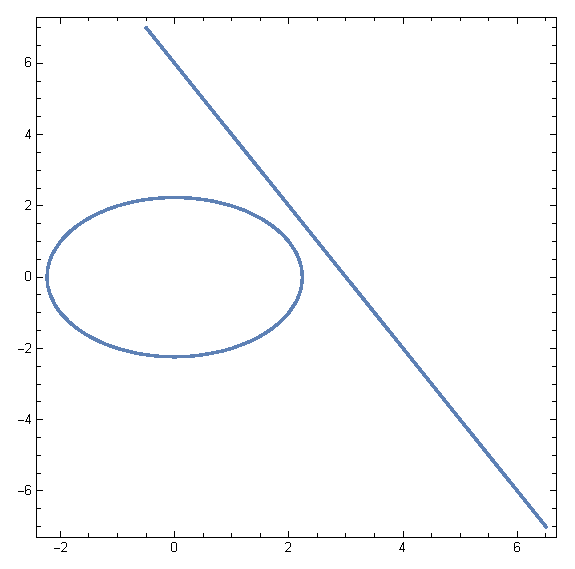
\includegraphics{optimization_kuhn_tucker_gr1.eps}

Now look, it would have been easier to start from the plot. The first constraint says we need the solution to be INSIDE the circle, and the second
constraint says the solution must be below the straight line, but as the circle IS BELOW the straight line, any solution in the circle is also satisfying
the second constraint. That{'}s why we did find a local minimum. The sad part of the story is that our local minimum was a saddle path, and therefore
we cannot say anything about its optimality a priore, so to let{'}s check the graph;

\tiny
\begin{doublespace}
\noindent\(\pmb{\text{Show}\left[\text{Plot3D}\left[f[x,y],\{x,-3,3\},\{y,-3,3\},\text{MeshFunctions}\to \left\{\text{$\#$1}^2+\text{$\#$2}^2\&\right\},\text{Mesh}\to
\{\{5\}\}\right],\text{Graphics3D}[\{\text{Red},\text{PointSize}[0.05],\text{Point}[\text{Append}[\{1,2\},f[1,2]]]\}]\right]}\)
\end{doublespace}
\normalsize
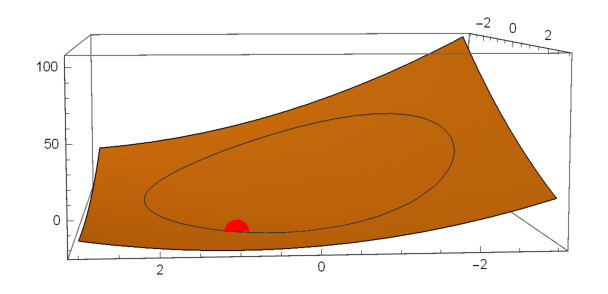
\includegraphics{optimization_kuhn_tucker_gr2.eps}

So we verify this is a minimum that satisfies both constraints (the red dot).

To see the code with small font size copy and paste in word for example, the only relevant thing is that it is within the page.

If you put the code in mathematica it gets more fun because you can ``move'' the last plot in 360 degrees.
